\subsubsection{UC15 - Gestione transazioni ed IVA}
\begin{figure}[H]
	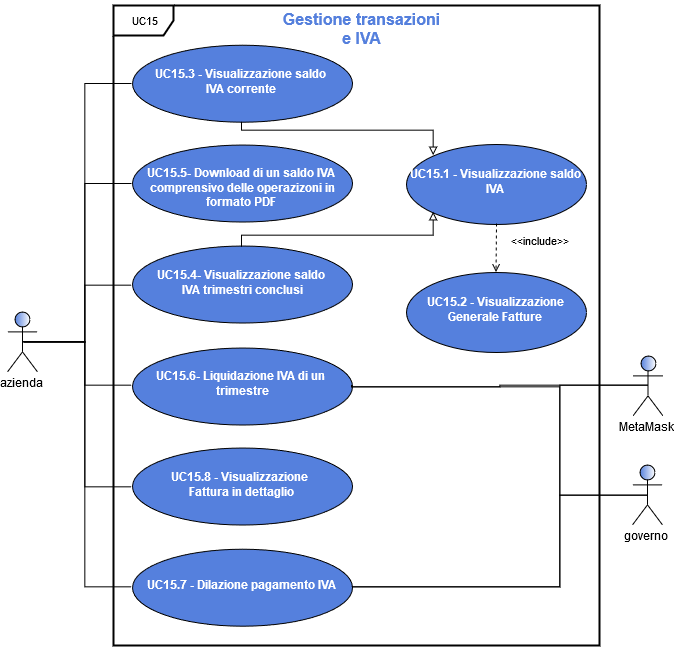
\includegraphics[width=12cm]{res/images/UC15-OK.png}
	\centering
	\caption{UC15 - Operazioni riguardanti la gestione dell'IVA}
\end{figure}
\begin{itemize}
	\item \textbf{Attori Primari}: azienda;
	\item \textbf{Descrizione}: alle aziende sono messe a disposizione diverse operazioni per gestire le transazioni e l'IVA:
	\begin{itemize}
		\item può visualizzare i saldi IVA di un periodo, comprendendo la visualizzazione di tutte le transazioni, rappresentate dalla rispettiva fattura, e del saldo finale [15.3 \& 15.4];
		\item per ogni fattura è disponibile la visualizzazione dettagliata [15.8];
		\item può scaricare le informazioni riguardanti un trimestre come sopra descritto sotto forma di documento PDF [15.5]; 
		\item in caso il saldo di un semestre risulti negativo (situazione di debito), l'azienda può procedere ad effettuare il versamento al governo [15.6] o può dilazionarlo\glosp [15.7];
	\end{itemize}
	\item \textbf{Scenario principale}: l'utente visualizza e svolge alcune operazioni per gestire l'IVA, gli ordini e le fatture;
	\item \textbf{Precondizione}: il sistema ha riconosciuto l'utente autenticato come azienda, e mette a disposizione tutte le pagine necessarie alla visualizzazione e gestione delle fatture e dell'IVA;
	\item \textbf{Postcondizione}: l'azienda ha visualizzato e/o svolto delle operazioni riguardanti fatture ed IVA.
\end{itemize} 
\subsubsection{UC15.1 - Visualizzazione saldo IVA}
\begin{itemize}
	\item \textbf{Attori Primari}: azienda;
	\item \textbf{Descrizione}: l'azienda può visualizzare il saldo IVA relativo ad un trimestre. In particolare può visualizzare il saldo:
	\begin{itemize}
		\item del trimestre corrente [15.3];
		\item di un trimestre concluso [15.4];
	\end{itemize}
	Il saldo conterrà tutte le fatture relative agli acquisti e le vendite che hanno determinato il suo valore, oltre al valore stesso;
	\item \textbf{Scenario principale}: l'utente visualizza il saldo relativo ad un trimestre. In particolare:
	\begin{enumerate}[label=\alph*.]
		\item seleziona da un menù a tendina uno dei trimestri disponibili;
		\item del trimestre scelto viene visualizzata la relativa lista delle fatture riguardanti gli ordini; 
	\end{enumerate}
	\item \textbf{Inclusioni}: 
	\begin{itemize}
		\item \textbf{UC15.2}: visualizzazione generale delle fatture, ovvero il mostrare la lista delle fatture nel saldo;
	\end{itemize}
	\item \textbf{Specializzazioni}: 
	\begin{itemize}
		\item \textbf{UC15.3}: visualizzazione saldo IVA corrente;
		\item \textbf{UC15.4}:  visualizzazione saldo IVA di un trimestre concluso;
	\end{itemize}
	\item \textbf{Precondizione}: il sistema ha riconosciuto l'utente autenticato come azienda, e mette a disposizione le pagine per visualizzazione dei saldi dei semestri IVA. L'utente ha selezionato un trimestre tra quelli disponibili;
	\item \textbf{Postcondizione}: l'azienda ha visualizzato il saldo IVA riguardante il trimestre scelto ed è a conoscenza dalla situazione di debito o credito verso il governo.
\end{itemize} 
\subsubsection{UC15.2 - Visualizzazione generale fattura}
\begin{itemize}
	\item \textbf{Attori Primari}: azienda;
	\item \textbf{Descrizione}: per ogni fattura l'utente può visualizzare i seguenti campi:
	\begin{itemize}
		\item numero identificativo;
		\item data;
		\item nome dell'azienda venditrice;
		\item nome dell'azienda cliente;
		\item importo totale dell'ordine;
		\item IVA a credito/debito derivante dalla transazione;
	\end{itemize}
	\item \textbf{Scenario principale}: l'utente visualizza una fattura, riguardante i propri  acquisti o le vendite;
	\item \textbf{Precondizione}: l'azienda sta visualizzando una pagina che richiede la visualizzazione dei dati generali di una fattura;
	\item \textbf{Postcondizione}: l'azienda ha visualizzato i dati relativi alla fattura.
\end{itemize}


\subsubsection{UC15.3 - Visualizzazione saldo IVA corrente}
\begin{itemize}
	\item \textbf{Attori Primari}: azienda;
	\item \textbf{Descrizione}: l'azienda può visualizzare il saldo parziale relativo al trimestre corrente, non ancora concluso. Non sono previste particolari operazioni per questa visualizzazione;
	\item \textbf{Scenario principale}: l'utente visualizza il saldo parziale relativo al trimestre corrente;
	\item \textbf{Precondizione}: l'utente ha selezionato la visualizzazione del saldo relativo al trimestre corrente;
	\item \textbf{Postcondizione}: l'azienda ha visualizzato il saldo IVA parziale riguardante il trimestre corrente ed è a conoscenza dall'attuale parziale situazione di debito o credito verso il governo.
\end{itemize} 

\subsubsection{UC15.4 - Visualizzazione saldo IVA trimestri conclusi}
\begin{itemize}
	\item \textbf{Attori Primari}: azienda;
	\item \textbf{Descrizione}: l'azienda può visualizzare la lista degli ordini relativi ad un trimestre IVA già concluso. Può inoltre leggerne lo stato, ovvero sapere se i pagamenti a debito o credito con il governo sono stati saldati oppure no. In caso di stato di debito relativo ad un trimestre, viene resa disponibile la data ultima per il versamento IVA, la possibilità di effettuare il pagamento, e quella di dilazionarlo;
	\item \textbf{Scenario principale}: l'utente visualizza la lista delle operazioni riguardanti  un saldo IVA relativo ad un trimestre concluso. Per ognuno di essi ottiene l'informazione sullo stato del pagamento del saldo IVA, assieme alle operazioni che possono essere effettuate su di esso;
	\item \textbf{Precondizione}: l'utente ha selezionato la visualizzazione del saldo relativo ad un trimestre concluso;
	\item \textbf{Postcondizione}: l'azienda ha visualizzato il saldo IVA riguardante un trimestre concluso, assieme alle possibili operazioni da effettuare.
\end{itemize} 

\subsubsection{UC15.5 - Download di un saldo IVA comprensivo delle operazioni in formato PDF}
\begin{itemize}
	\item \textbf{Attori Primari}: azienda;
	\item \textbf{Descrizione}: alle aziende è offerta la possibilità di scaricare le operazioni riguardanti un saldo trimestrale IVA nel formato PDF;
	\item \textbf{Scenario principale}: l'utente, dopo aver individuato il saldo desiderato, scarica, in formato PDF, l'elenco delle operazioni riguardanti il periodo trimestrale IVA selezionato;
	\item \textbf{Inclusioni}:
	\begin{itemize}
		\item \textbf{UC15.2}: l'azienda, per poter scaricare le informazioni riguardanti le operazioni di un trimestre IVA concluso, deve aver prima visualizzato un trimestre IVA concluso [UC15.4];
	\end{itemize}
	\item \textbf{Precondizione}: l'azienda ha selezionato un saldo IVA riguardante un trimestre concluso, ed ha espresso la volontà di scaricare i dati relativi agli ordini riguardanti il periodo cliccando l'apposito pulsante;
	\item \textbf{Postcondizione}: l'azienda ha scaricato il documento PDF contenente tutti i dati riguardanti gli ordini del periodo trimestrale IVA selezionato.
\end{itemize} 

\subsubsection{UC15.6 - Liquidazione IVA di un trimestre}
\begin{itemize}
	\item \textbf{Attori Primari}: azienda;
	\item \textbf{Attori Secondari}: governo;
	\item \textbf{Descrizione}: l'azienda può versare l'ammontare dovuto al governo, relativo ad un saldo trimestrale IVA concluso che risultasse in stato di debito verso il governo;
	\item \textbf{Scenario principale}: l'utente, dopo aver individuato il saldo desiderato, effettua il versamento dell'ammontare dovuto allo stato premendo sull'apposito pulsante. Per effettuare il versamento viene utilizzato MetaMask\glo;
	\item \textbf{Inclusioni}:
	\begin{itemize}
		\item \textbf{UC15.4}: l'azienda per poter saldare il debito riguardante un semestre IVA concluso deve averlo prima visualizzato;
	\end{itemize}
	\item \textbf{Precondizione}: l'utente ha visualizzato un particolare saldo trimestrale IVA concluso. L'utente è in stato di debito verso il governo relativamente al saldo IVA trimestrale considerato. L'utente desidera saldare il debito relativo al suddetto trimestre, e dunque clicca sul pulsante dedicato;
	\item \textbf{Postcondizione}: l'azienda ha effettuato il pagamento verso il governo. Viene aggiornato lo stato del trimestre IVA, che ora risulta saldato, sia nella visualizzazione da parte dell'azienda che da parte del governo.
\end{itemize} 

\subsubsection{UC15.7 - Dilazione pagamento IVA}
\begin{itemize}
	\item \textbf{Attori Primari}: azienda;
	\item \textbf{Attori Secondari}: governo;
	\item \textbf{Descrizione}: l'azienda può dilazionare\glosp il pagamento dovuto al governo, relativo ad un saldo trimestrale IVA concluso che risultasse in stato di debito verso il governo;
	\item \textbf{Scenario principale}: l'utente, dopo aver individuato il saldo desiderato:
	\begin{enumerate}[label=\alph*.]
		\item sceglie da un menù a tendina di quanti mesi dilazionare\glosp il pagamento, se tale opzione risulta disponibile;
		\item conferma la dilazione\glosp del versamento dell'ammontare dovuto allo stato premendo sull'apposito pulsante. Per effettuare il versamento viene utilizzato MetaMask\glo;
	\end{enumerate}
	 
	\item \textbf{Inclusioni}:
	\begin{itemize}
		\item \textbf{UC15.4}: l'azienda per poter dilazionare\glosp il pagamento del debito riguardante un trimestre IVA concluso deve averlo prima visualizzato;
	\end{itemize}
	\item \textbf{Precondizione}: l'utente ha visualizzato un particolare saldo trimestrale IVA concluso. L'utente è in stato di debito verso il governo relativamente al saldo IVA trimestrale considerato. L'utente desidera dilazionare\glosp il debito relativo al suddetto periodo; 
	\item \textbf{Postcondizione}: l'azienda ha effettuato la dilazione\glosp del pagamento verso il governo.
\end{itemize} 

\subsubsection{UC15.8 - Visualizzazione fattura in dettaglio}

\begin{itemize}
	\item \textbf{Attori Primari}: azienda;
	\item \textbf{Descrizione}: l'azienda può leggere tutti i dettagli di una fattura. In essa devono essere presenti tutti i seguenti campi:
	\begin{itemize}
		\item data della fattura;
		\item numero identificativo della fattura;
		\item la data dell'ordine relativo alla fattura;
		\item il numero identificativo dell'ordine relativo alla fattura;
		\item visualizzazione dei beni in formato fattura, ovvero UC5 con due campi aggiuntivi per ogni prodotto, ovvero il prezzo netto\glosp e la aliquota IVA imposta;
		\item l'importo totale dell'ordine;
		\item il nome dell'azienda emittente;
		\item la partita IVA dell'azienda emittente;
		\item informazioni relative all'acquirente:
		\begin{itemize}
			\item nel caso il cliente fosse un'\textbf{azienda}:
			\begin{itemize}
				\item il nome dell'azienda destinataria;
				\item la partita IVA dell'azienda destinataria;
			\end{itemize}
			\item nel caso il cliente fosse un \textbf{cittadino}:
			\begin{itemize}
				\item il nome;
				\item il cognome;
			\end{itemize}
		\end{itemize}
		
		\item indirizzo di spedizione dell'ordine;
	\end{itemize}
	\item \textbf{Scenario principale}: l'azienda seleziona una fattura da una lista e può leggere tutti i dettagli di tale fattura;
	\item \textbf{Inclusioni}:
	\begin{itemize}
		\item \textbf{UC15.2}: per poter accedere ai dettagli di una particolare fattura è necessario selezionarla da una delle liste disponibili nei saldi;
	\end{itemize}
	\item \textbf{Precondizione}: il sistema ha riconosciuto l'utente autenticato come azienda, l'utente ha espresso la volontà di visualizzare i dettagli di una specifica fattura;
	\item \textbf{Postcondizione}: l'azienda ha visualizzato i dettagli della fattura selezionata.
\end{itemize} 


